% \documentclass[bwprint]{cumcmthesis} %去掉封面与编号页
\documentclass[withoutpreface,bwprint]{cumcmthesis} %去掉封面与编号页
\newcommand{\diff}{\mathop{}\!\mathrm{d}} % 正体微分符号

\usepackage{graphicx}       % 用于插入图片
\usepackage{subcaption} 
\usepackage{algorithm}
\usepackage{algorithmic} % 导言区需添加这两个宏包
\usepackage{comment}  

\usepackage{booktabs}
\usepackage{tabularx}
\usepackage{float}
\usepackage[numbers]{natbib}
\usepackage{threeparttable} % 表,图注
\usepackage[table]{xcolor}      % 颜色选项


\title{基于统计学习方法的NIPT时点选择与胎儿的异常判定决策模型}
\tihao{C}
\baominghao{1234}
\schoolname{中原工学院}
\membera{杨帅博}
\memberb{洪宜昕}
\memberc{宋诗昊}
\supervisor{魏冰蔗}
\yearinput{2025}
\monthinput{09}
\dayinput{07}


\begin{document}

% 标题
\maketitle
\nocite{*}
\bibliographystyle{gbt7714-numerical}

\begin{abstract}

    \textbf{针对问题一,}

    \textbf{针对问题二,}

    \textbf{针对问题三,}

    \textbf{针对问题四,}

    \keywords{}
\end{abstract}

% 问题背景与重述
\section{问题重述}

\subsection{问题背景}
NIPT是一种通过采集母体血液、检测胎儿的游离DNA 片段、分析胎儿染色体是否存在异常的产前检测技术,目的是通过早期检测确定胎儿的健康状况。根据临床经验,畸型胎儿主要有唐氏综合征、爱德华氏综合征和帕陶氏综合征,这三种体征分别由胎儿21 号、18 号和 13 号“染色体游离 DNA 片段的比例”是否异常决定。NIPT 的准确性主要由胎儿性染色体浓度判断。通常孕妇的孕期在 10 周~25 周之间可以检测胎儿性染色体浓度,且如果男胎的 Y 染色体浓度达到或高于 4\%、女胎的 X 染色体浓度没有异常,则可认为 NIPT 的结果是基本准确的,否则难以保证结果准确性要求。同时,实际中应尽早发现不健康的胎儿,否则会带来治疗窗口期缩短的风险,早期发现风险较低;中期发现风险高;晚期发现风险极高。实践表明,男胎 Y 染色体浓度与孕妇孕周数及其身体质量指数(BMI)紧密相关。通常根据孕妇的
BMI 值进行分组分别确定 NIPT 的时点。由于每个孕妇的年龄、BMI、孕情等存在个体差异,对所有孕妇采用简单的经验分组和统一的检测时点进行 NIPT,会对其准确性产生较大影响。因此,依据 BMI 对孕妇进行合理分组,确定各不同群组的最佳 NIPT 时点,可以减少某些孕妇因胎儿不健康而缩短治疗窗口期所带来的潜在风险。为了研究各类孕妇群体合适的 NIPT 时点,并对检测的准确性进行分析,附件给出了某地区孕妇的 NIPT 数据。在实际检测中,经常会出现测序失败的情况。同时为了增加检测结果的可靠性,对某些孕妇有多次采血多次检测或一次采血多次检测的情况。试利用附件提供的数据建立数学模型研究如下问题:

\subsection{问题提出}

\textbf{问题1:}
分析胎儿 Y 染色体浓度与孕妇的孕周数和 BMI 等指标的相关特性,给出相应的关系模型,并检验其显著性。

\textbf{问题2:}
男胎孕妇的 BMI 是影响胎儿 Y 染色体浓度的最早达标时间的主要因素。要求对男胎孕妇的 BMI 进行合理分组,给出每组的 BMI 区间和最佳 NIPT时点,使得孕妇可能的潜在风险最小,并分析检测误差对结果的影响。

\textbf{问题3:}
综合考虑身高、体重、年龄等等多种因素对男胎 Y 染色体浓度达标时间的影响、检测误差和胎儿的 Y 染色体浓度达标比例,根据男胎孕妇的 BMI,给出合理分组以及每组使得孕妇潜在风险最小的最佳 NIPT 时点,并分析检测误差对结果的影响。

\textbf{问题4:}
以女胎孕妇的 21号、18 号和 13 号染色体非整倍体(AB 列)为判定女胎是否异常结果,综合考虑 X 染色体及上述染色体的 Z 值、GC含量、读段数及相关比例、BMI 等因素,给出女胎异常的判定方法。





% 问题分析
\section{问题分析}
\subsection{问题一分析}

\subsection{问题二分析}

\subsection{问题三分析}

\subsection{问题四分析}


% 模型假设
\section{模型假设}

\begin{enumerate}
    \item 
    \item 
    \item 
\end{enumerate}



% 符号说明
\section{符号说明}

% 表结构
\begin{table}[h]
    \centering
    \begin{tabular}{ll}
        \toprule
        符号 & 说明 \\
        \midrule
        $Y$ & Y 染色体浓度(\%) \\
        $W$ & 孕周数(周) \\
        $B$ & 孕妇 BMI(kg/m²) \\
        $A$ & 孕妇年龄(岁) \\
        $G$ & GC 含量(\%) \\
        $R$ & 原始读段数 \\
        $Z_i$ & 第 $i$ 号染色体 Z 值 \\
        $\beta_0, \beta_1, \dots$ & 回归模型参数 \\
        $r$ & 相关系数 \\
        $p$ & 显著性 p 值 \\
        $R^2$ & 模型解释方差比例 \\
        \bottomrule
    \end{tabular}
    \caption{符号说明表}
    \label{tab:symbols}
\end{table}

% 模型建立与求解
\section{模型建立与求解}

\subsection{问题一模型的建立与求解}
\subsubsection{数据预处理}
预处理步骤:
\begin{enumerate}
    \item \textbf{缺失值处理}:数值列(如 BMI、读段数)用中位数填充,类别列(如非整倍体)用众数(T18)填充,末次月经(1.11\% 缺失)用众数“2022-12-28”填充。
    \item \textbf{异常值处理}:使用 Z-score ($|Z| > 3$) 检测极端值(如 Y 浓度异常 8 个),标记但未移除,保留生理合理范围。
    \item \textbf{孕周转换}:将“检测孕周”转换为数值(保留两位小数),计算孕周 = (检测日期 - 末次月经)/7,过滤孕周 10-40 周。
    \item \textbf{数据清洗结果}:去重后 1082 条,有效样本 1076 条。
\end{enumerate}

异常值统计表:

\begin{table}[h]
    \centering
    \begin{tabular}{lc}
        \toprule
        指标 & 极端异常值数量 \\
        \midrule
        年龄 & 11 \\
        BMI & 14 \\
        Y 浓度 & 8 \\
        GC 含量 & 13 \\
        ... (总计) & 167 \\
        \bottomrule
    \end{tabular}
    \caption{异常值统计}
    \label{tab:outliers}
\end{table}

预处理提升数据质量,保持原始数据完整性。

\subsection{相关性分析}

分析 Y 染色体浓度 ($Y$) 与孕周 ($W$)、BMI ($B$)、GC 含量、原始读段数的关系,计算皮尔逊、斯皮尔曼和肯德尔相关系数,显著性以 $p < 0.05$ 为阈值。

计算结果(有效样本 1076):
\begin{itemize}
    \item $Y$ 与 $W$:皮尔逊 $r=0.077$ ($p=0.0110^*$),弱正相关。
    \item $Y$ 与 $B$:皮尔逊 $r=-0.158$ ($p=0.0000^{***}$),弱负相关。
    \item $Y$ 与 GC 含量:$r=-0.022$ ($p=0.4666$ ns),无显著相关。
    \item $Y$ 与原始读段数:$r=-0.111$ ($p=0.0003^{***}$),弱负相关。
\end{itemize}

皮尔逊相关效果最佳,整体弱相关($|r|<0.2$)但显著,支持线性模型。

\begin{figure}[h]
    \centering
    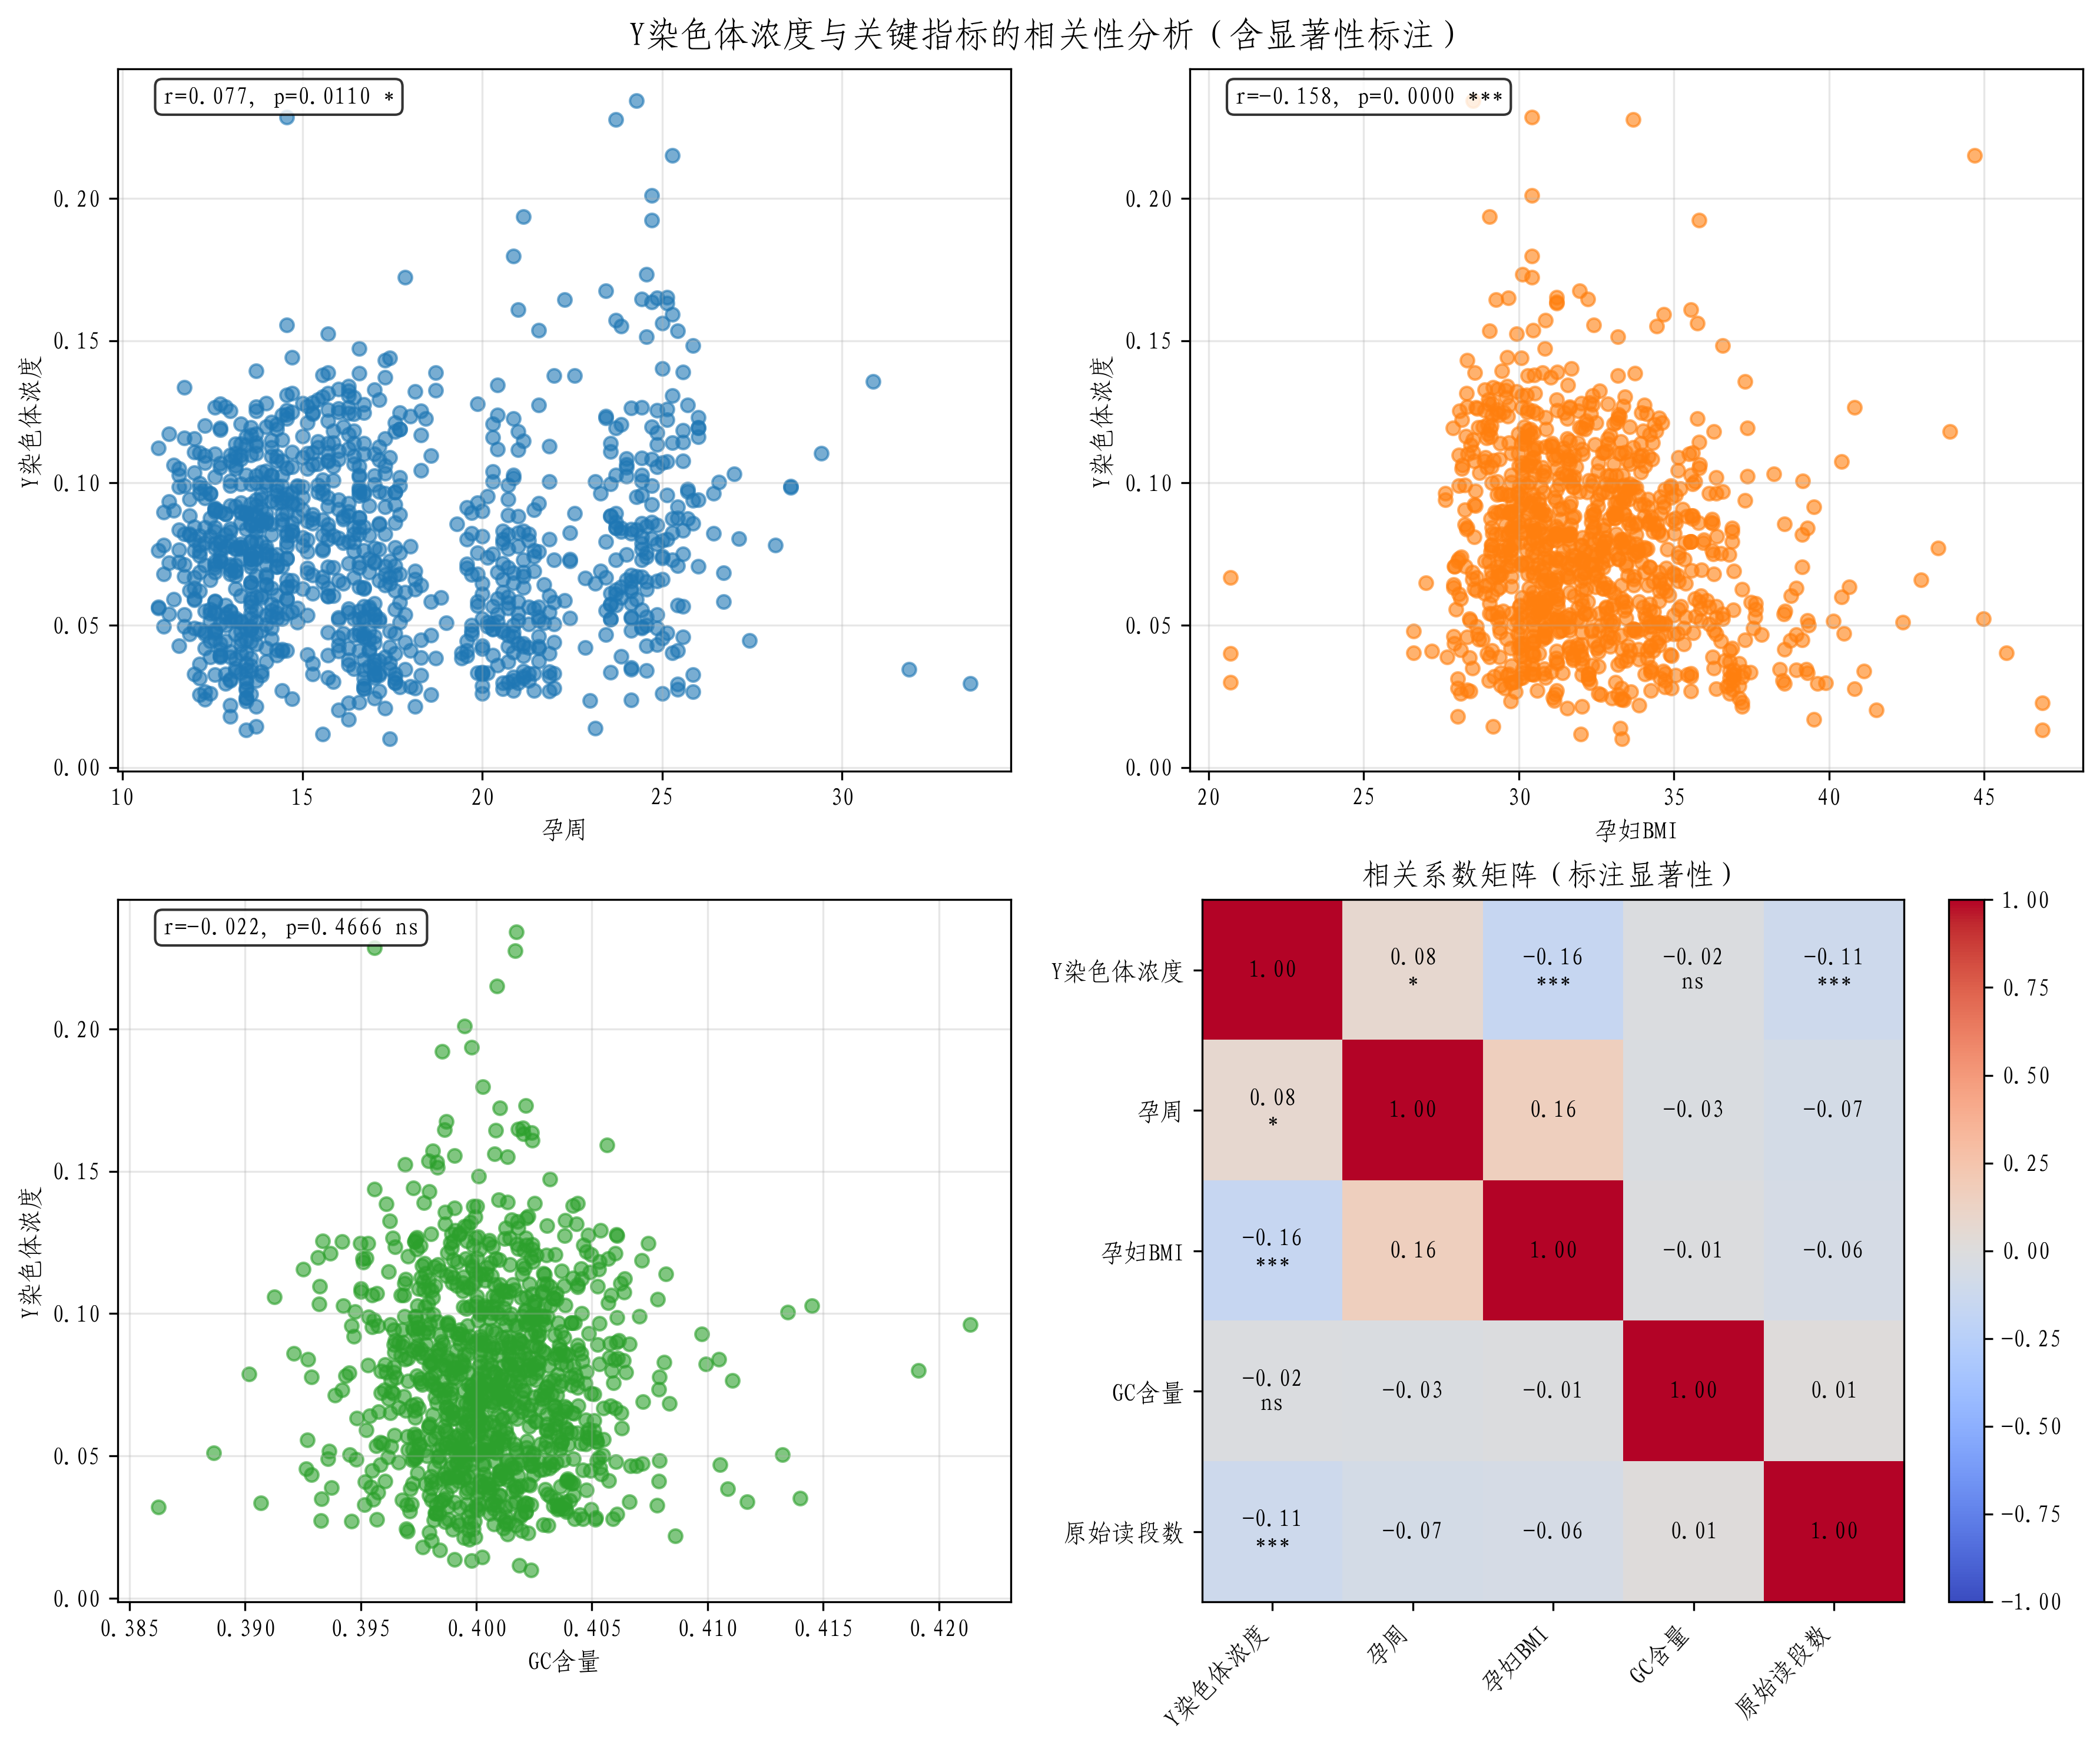
\includegraphics[width=0.8\textwidth]{../code/fig-1-1-y_chromosome_correlation_with_sig.png}
    \caption{Y 染色体浓度相关性分析}
    \label{fig:corr}
\end{figure}

\subsection{关系模型}

建立多元线性回归模型:$\log Y = \beta_0 + \beta_1 W + \beta_2 B + \beta_3 (W \times B) + \epsilon$。

模型结果(样本 1076):
\begin{itemize}
    \item $R^2 = 0.053$(调整 $R^2 = 0.050$),解释 5.3\% 方差。
    \item 参数:$\beta_0 = 3.9507$ ($p=0.000^{***}$),$\beta_1 = -0.0077$ ($p=0.114$ ns),$\beta_2 = -0.0628$ ($p=0.001^{**}$),$\beta_3 = 0.0003$ ($p=0.053$ ns)。
    \item F 统计 = 17.34 ($p=5.88e-11^{***}$),模型显著。
\end{itemize}

GAM 模型 $R^2 = 0.1698$,拟合优于线性模型。

\begin{figure}[h]
    \centering
    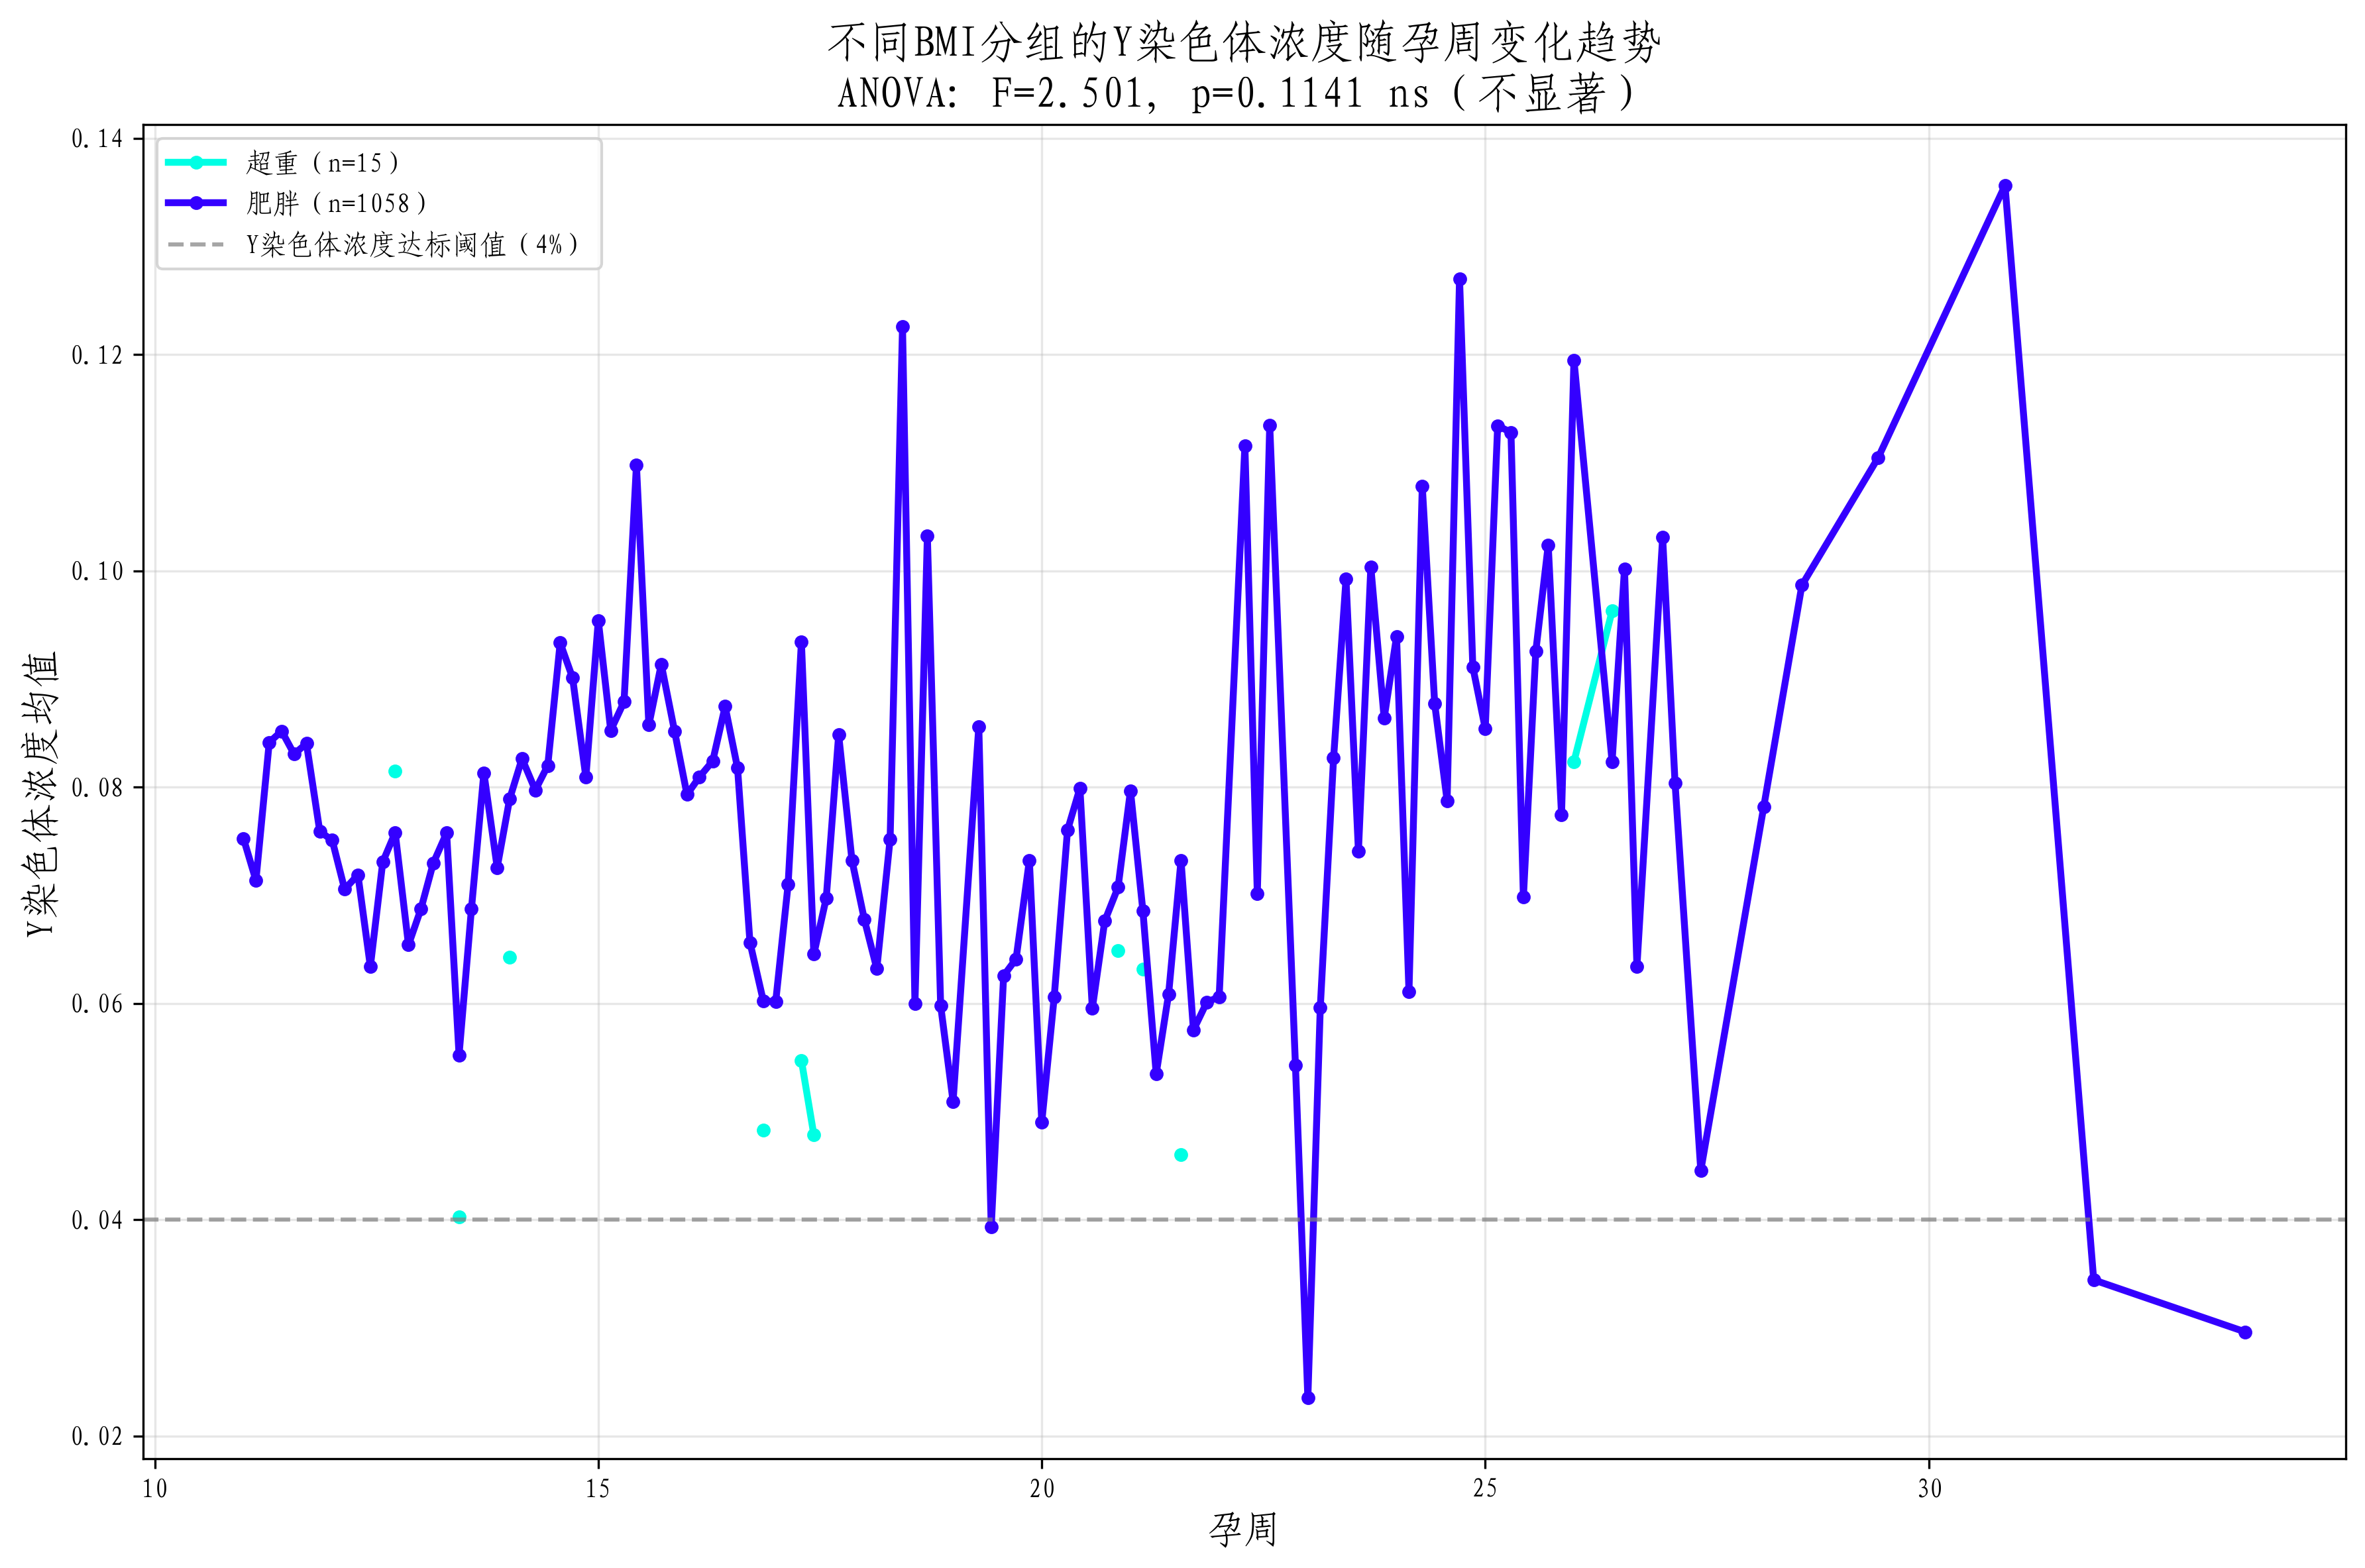
\includegraphics[width=0.8\textwidth]{../code/fig-1-2-y_chromosome_by_bmi_week_with_anova.png}
    \caption{BMI 分组趋势分析}
    \label{fig:trend}
\end{figure}

\subsection{显著性检验}

\begin{enumerate}
    \item \textbf{p 检验与 t 检验}:BMI 系数显著 ($p=0.001$),孕周和交互项不显著,整体 F 检验 $p<0.001$。
    \item \textbf{ANOVA 分组检验}:BMI 分组(超重 15、肥胖 1058),$F=2.501$ ($p=0.114$ ns),超重 vs 肥胖 $t=-2.217$ ($p=0.0427^*$)。
    \item \textbf{正态性检验}:Z 值非正态(13 号 $p<0.05$ 等),需非参数方法。
    \item \textbf{质量控制 ANOVA}:GC 含量 $F=6.336$ ($p=0.0120^*$),读段数 $F=4.083$ ($p=0.0436^*$),显著。
\end{enumerate}

\begin{figure}[h]
    \centering
    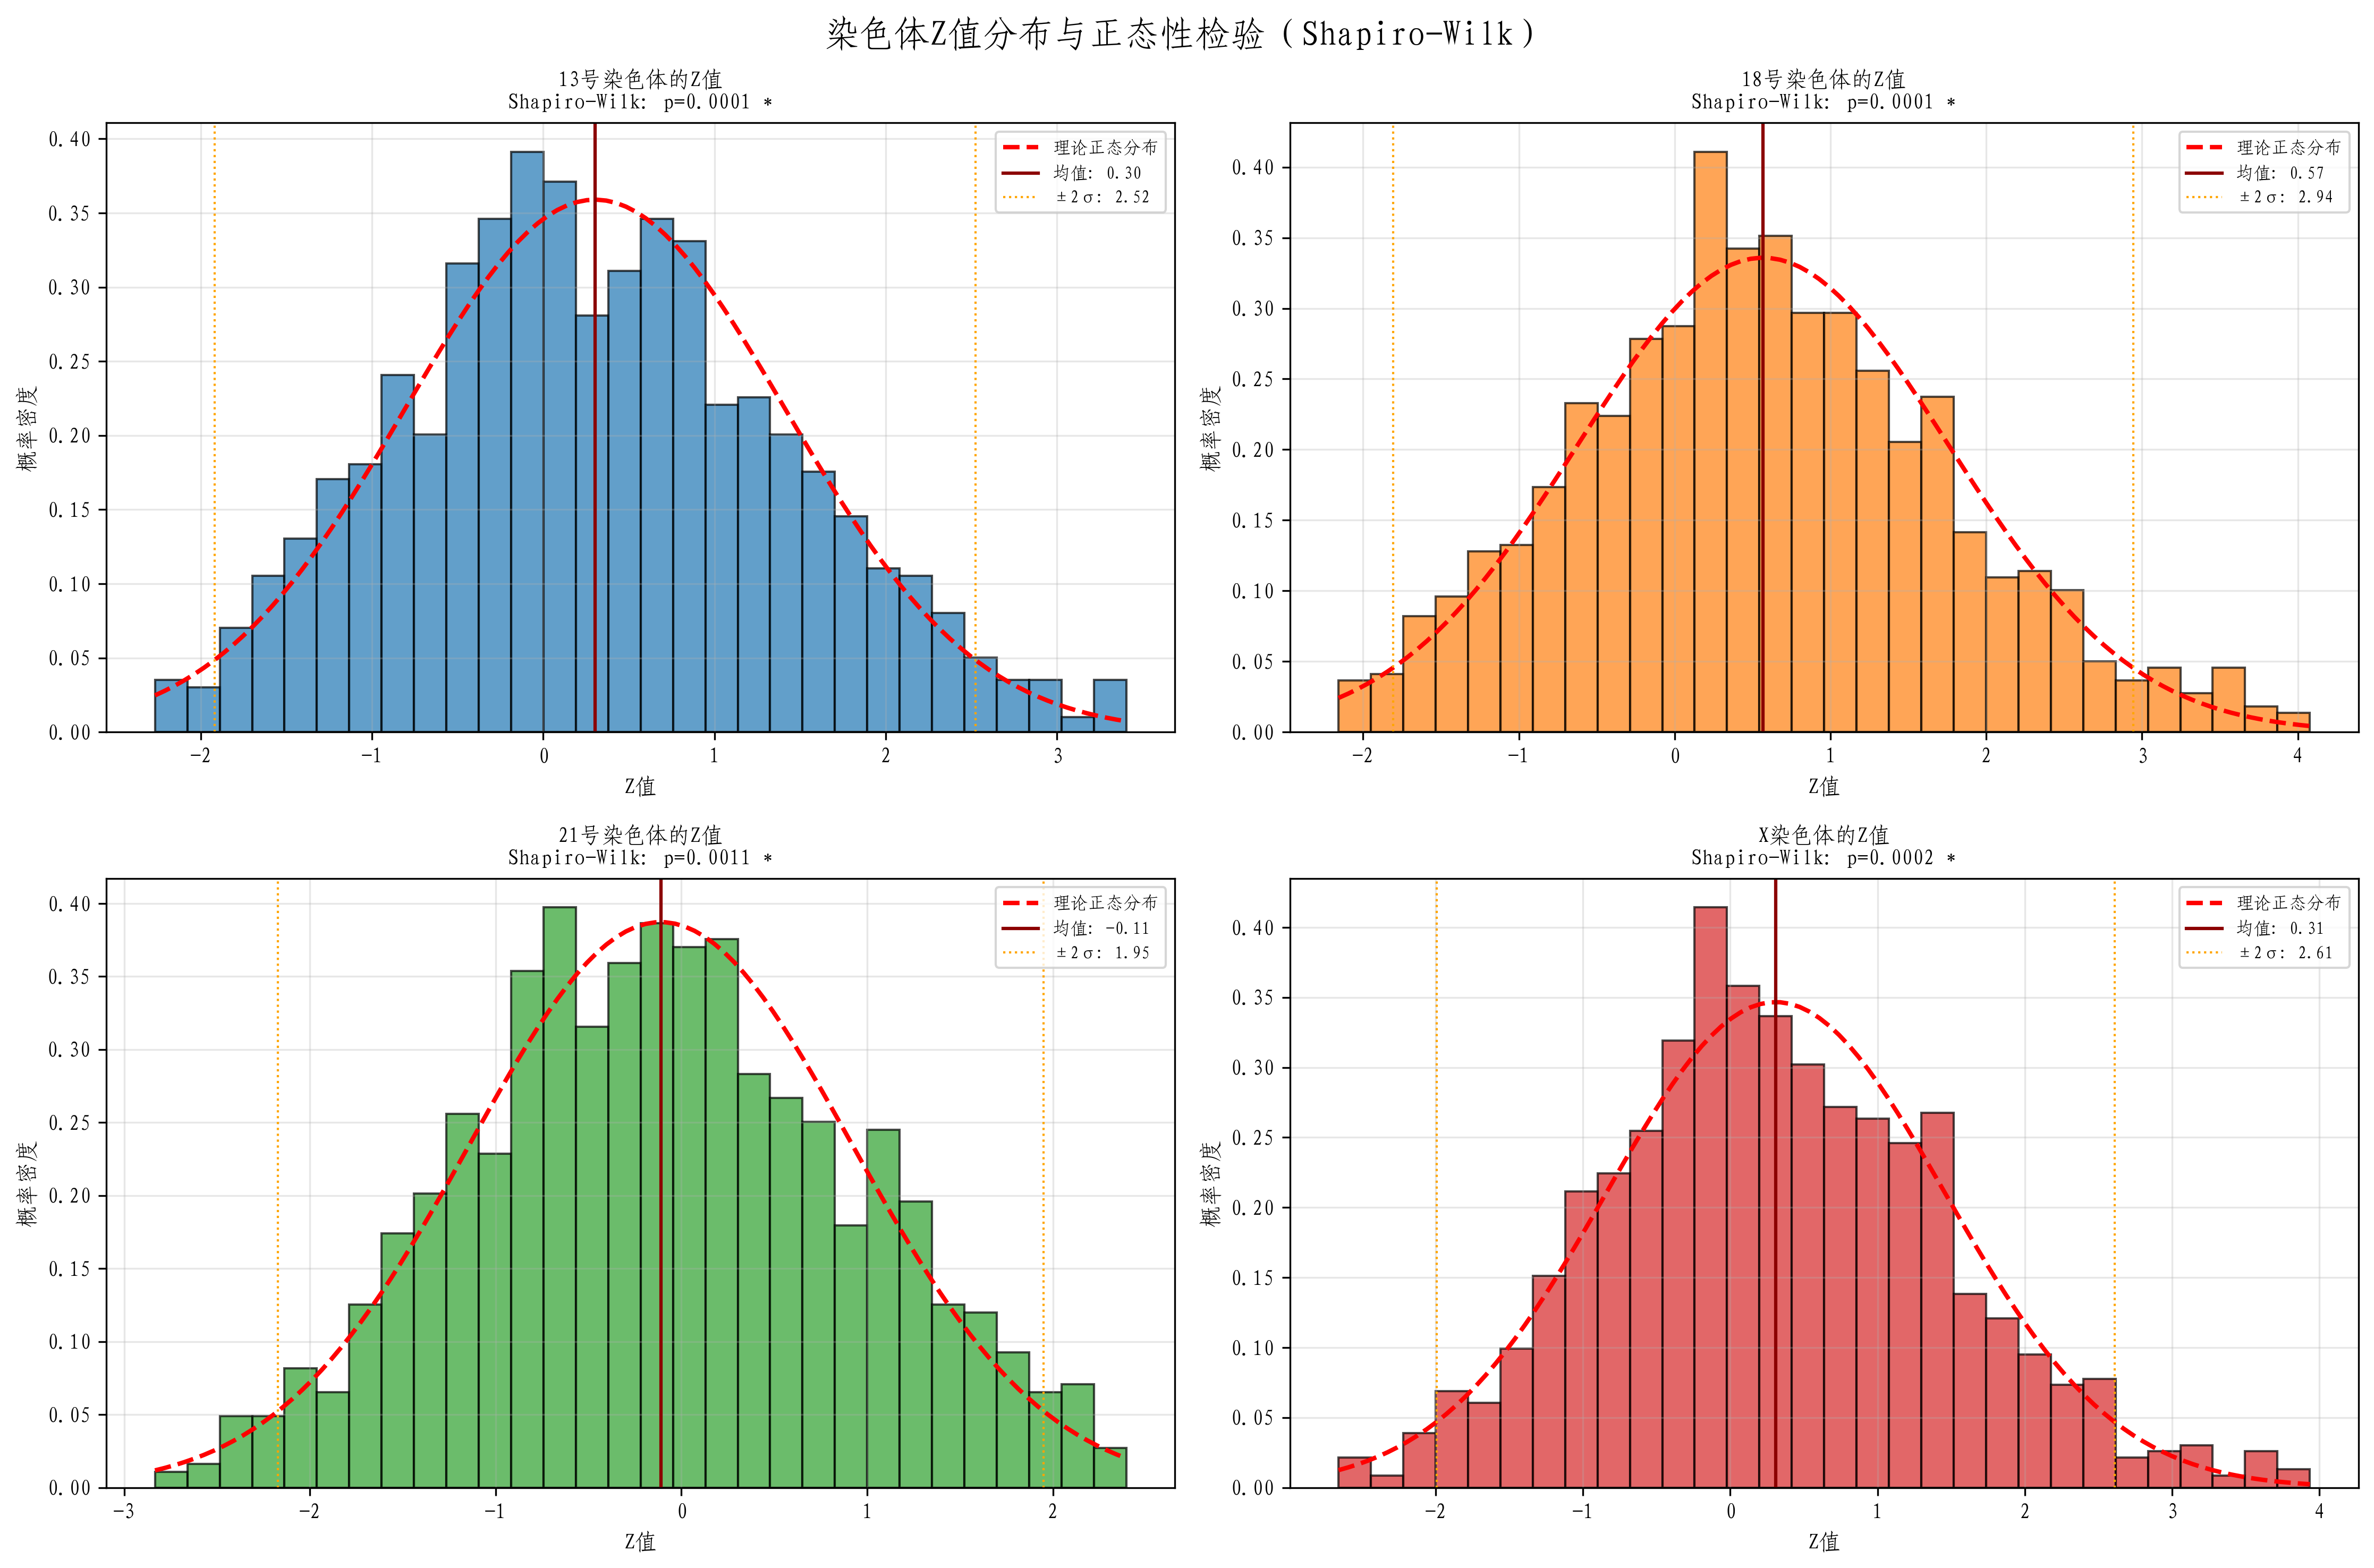
\includegraphics[width=0.8\textwidth]{../code/fig-1-3-chromosome_zvalue_distribution_with_normtest.png}
    \caption{Z 值分布与正态性检验}
    \label{fig:zdist}
\end{figure}

\begin{figure}[h]
    \centering
    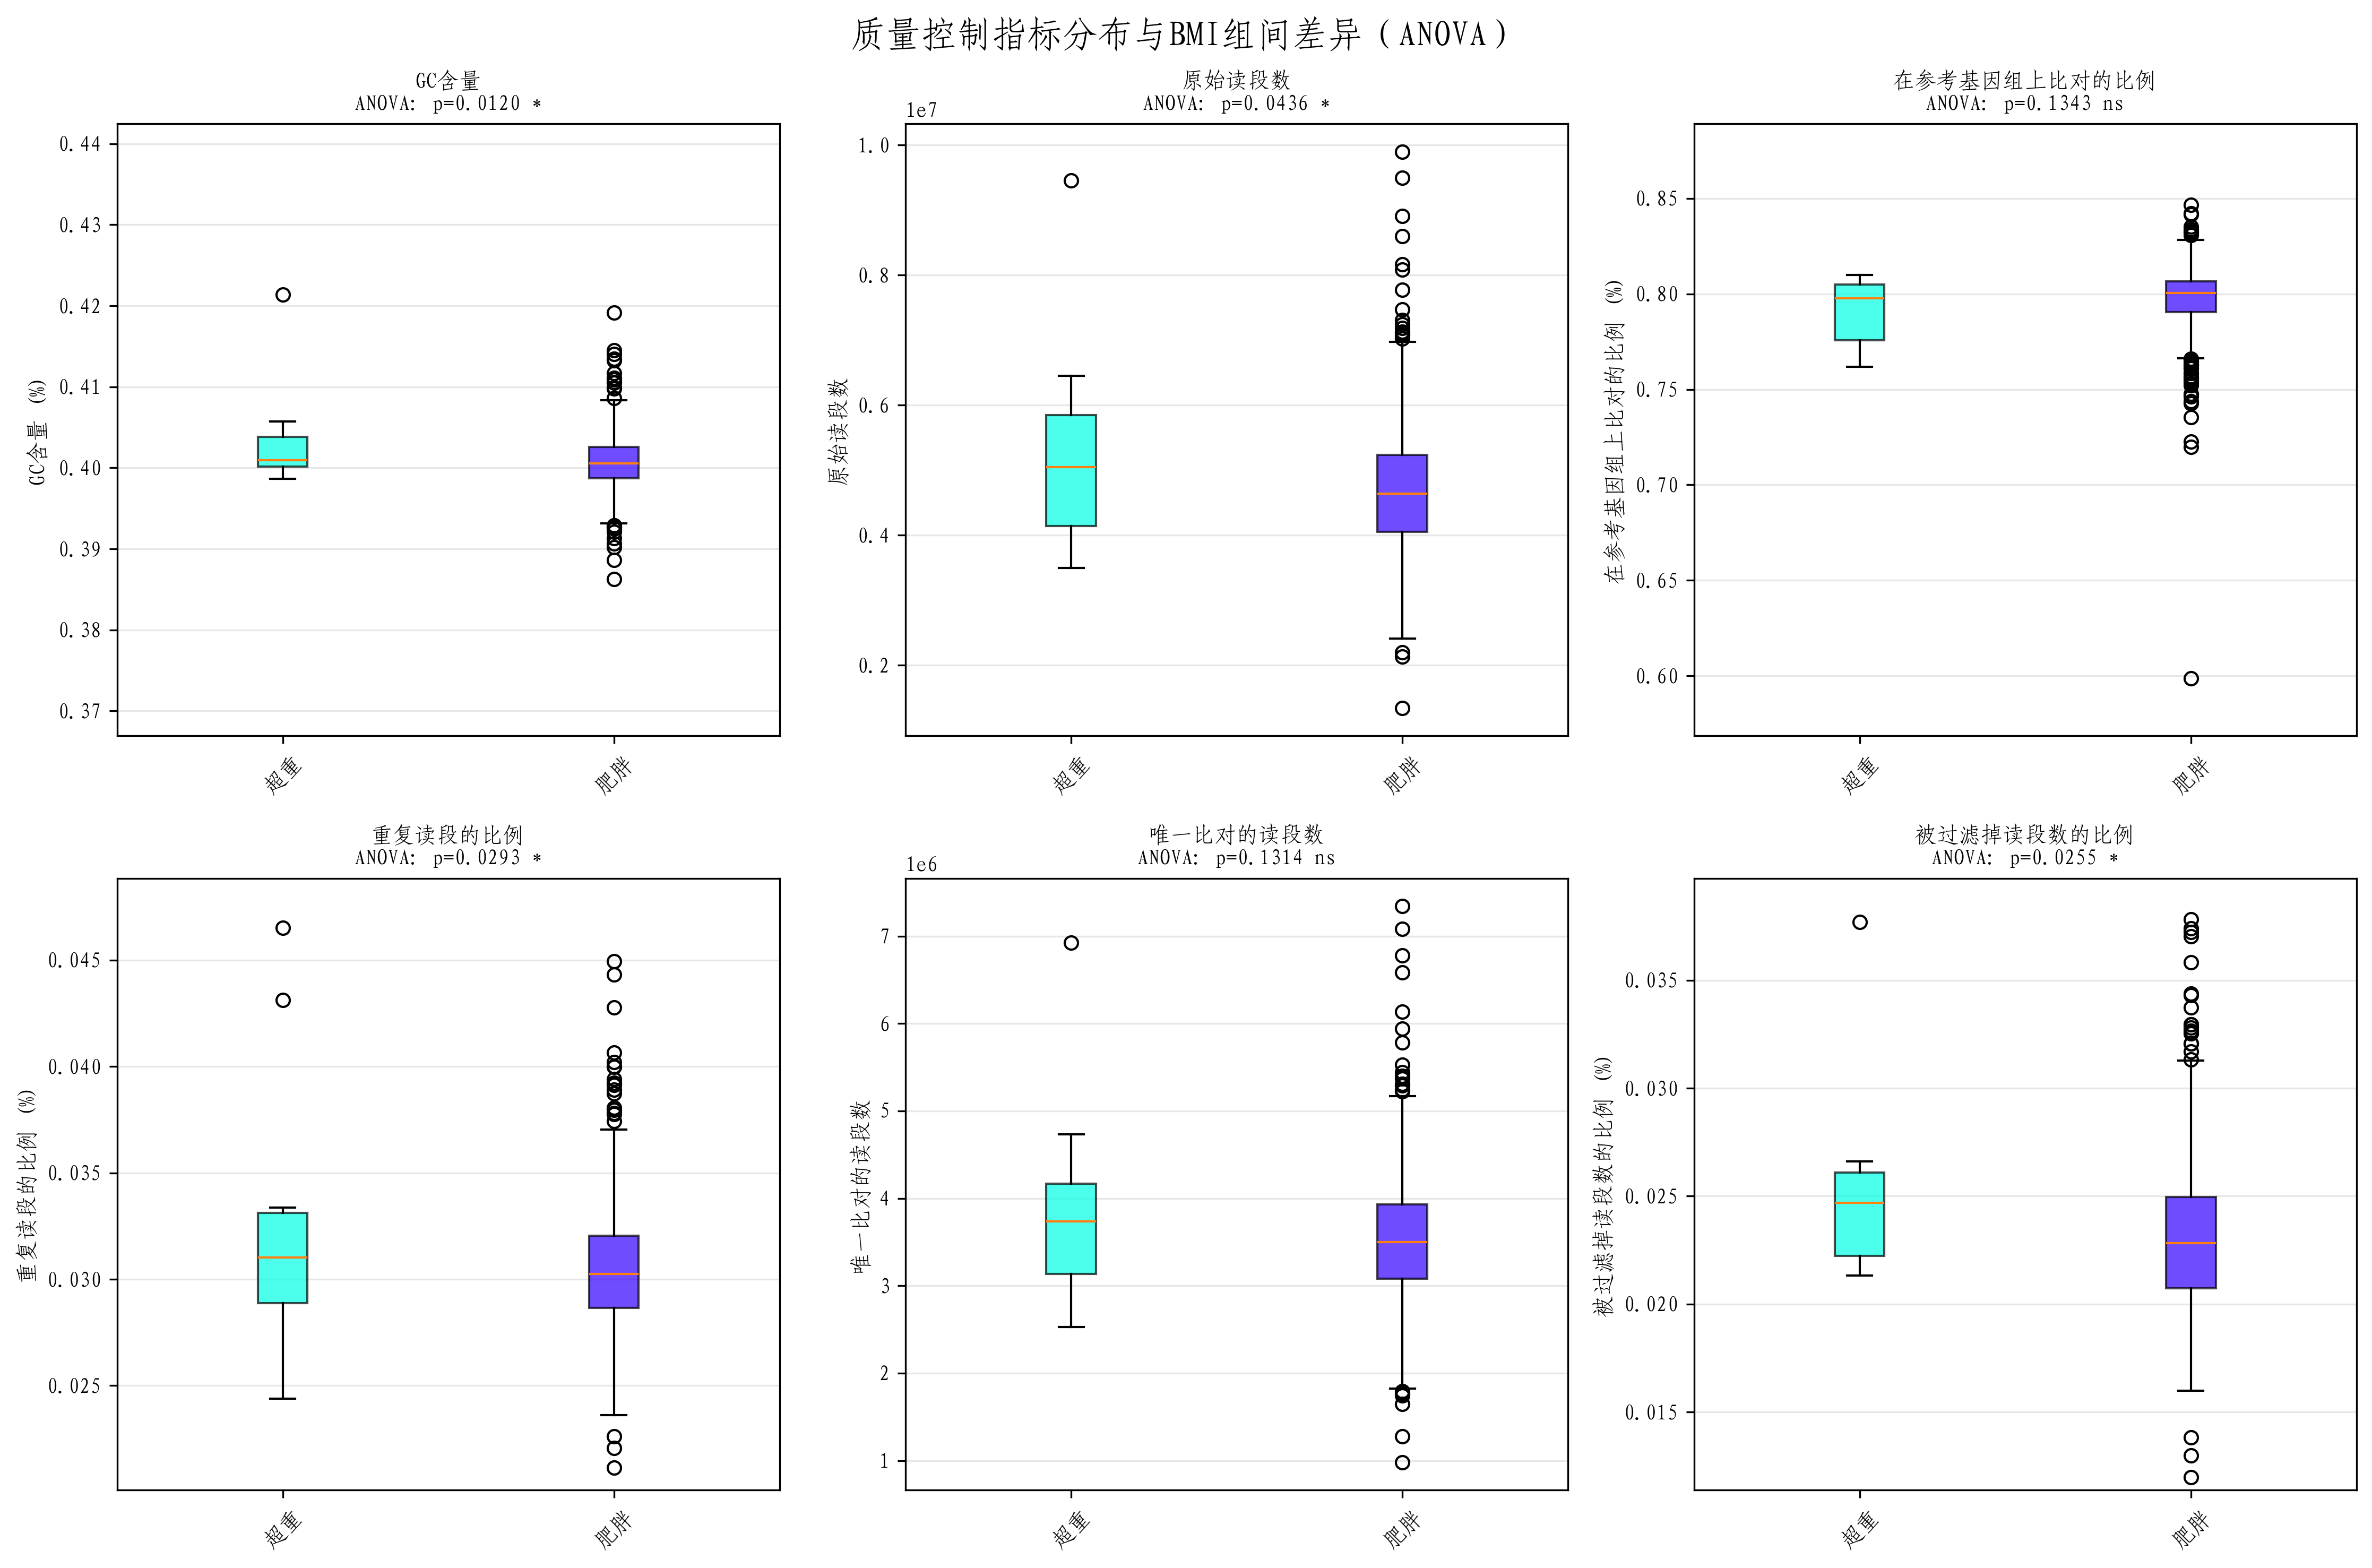
\includegraphics[width=0.8\textwidth]{../code/fig-1-4-quality_control_with_anova.png}
    \caption{质量控制指标分析}
    \label{fig:qc}
\end{figure}

\subsection{问题一小结}

$Y$ 与 $W$ 弱正相关 ($r=0.077$, $p=0.011$),与 $B$ 弱负相关 ($r=-0.158$, $p<0.001$)。回归模型 $\log Y = 3.9507 - 0.0077 W - 0.0628 B + 0.0003 (W \times B)$ ($R^2=0.053$),GAM 提升至 0.1698。BMI 影响显著,建议优化模型。




\subsubsection{相关性分析}

\subsubsection{显著性检验}

p检验t检验

散点图 热力图








\subsection{问题二模型的建立与求解}

\subsection{问题三模型的建立与求解}

\subsection{问题四模型的建立与求解}

% 模型评价
\section{模型评价}
\subsection{模型优点}

\subsection{模型缺点}

% 摘要
\bibliography{ref}

% 附录

\begin{appendices}
    % \section{附录名}
\end{appendices}

\end{document}